\icode{N23J-MM-CA-L2-261017-003}
\nceeID[9]{2023北京}{17}
如图所示，质量为\(m\)的小球\(A\)用一不可伸长的轻绳悬挂在\(O\)点，在\(O\)点正下方的光滑桌面上有一个与\(A\)完全相同的静止小球\(B\)，\(B\)距\(O\)点的距离等于绳长\(L\)。现将\(A\)拉至某一高度，由静止释放，\(A\)以速度\(v\)在水平方向和\(B\)发生正碰并粘在一起。重力加速度为\(g\)。求：
\begin{enumerate}
	\item \(A\)释放时距桌面的高度\(H\)。
	\item 碰撞前瞬间绳子的拉力大小\(F\)。
	\item 碰撞过程中系统损失的机械能\(\Delta E\)。
\end{enumerate}
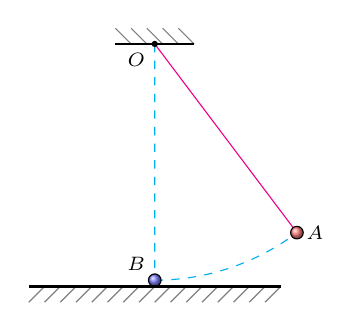
\begin{tikzpicture}[font=\scriptsize]
	\draw[dashed,cyan] (0,0)--(0,-3) (0,-3) arc(-90:-53:3);
	\draw[magenta] (0,0)--(-53:3)node[right,black]{\(A\)};
	\draw[ball color=red!50] (-53:3) circle(.08);
	\draw[ball color=blue!50] (0,-3)node[above left]{\(B\)} circle(.08);
	\foreach \x in {-1.6,-1.4,...,1.6}
		\draw[gray] (\x,-3.28)--++(.2,.2);
	\foreach \x in{-.5,-.3,...,.3}
		\draw[gray] (\x,.2)--++(.2,-.2);
	\draw[thick] (-1.6,-3.08)--(1.6,-3.08) (-.5,0)--(.5,0);
	\fill (0,0)node[below left]{\(O\)} circle(.04);
\end{tikzpicture}
\begin{answer}
	（1）\(\frac{v^2}{2g}\)（2）\(mg + m \frac{v^2}{L}\)（3）\(\frac{1}{4}mv^2\)
\end{answer}